\documentclass[12pt, a4paper]{ctexart}
\usepackage{geometry}
\geometry{left=2.5cm, right=2.5cm, top=3cm, bottom=3cm}
\usepackage{listings}
\usepackage{graphicx}
\usepackage{xcolor}
\usepackage{amsmath}
\usepackage{booktabs}
\usepackage{tikz}
\usetikzlibrary{positioning, arrows.meta}
\usepackage{float}

% Code snippet settings
\lstset{
    basicstyle=\ttfamily\small,
    frame=single,
    framesep=5pt,
    xleftmargin=10pt,
    xrightmargin=10pt,
    keywordstyle=\color{blue},
    commentstyle=\color{gray},
    breaklines=true
}

\begin{document}

% 封面
\begin{titlepage}
    \centering
    \vspace*{5cm}
    {\Huge\bfseries 实验报告\par}
    \vspace{2cm}
    {\Large 课程：数字逻辑与计算机组成实验\par}
    \vspace{1cm}
    {\Large 实验七：VGA 显示控制\par}
    \vspace{4cm}
    {\large 姓名：\underline{\makebox[4cm]{郑袭明}}\par}
    \vspace{1cm}
    {\large 学号：\underline{\makebox[4cm]{251502027}}\par}
    \vspace{1cm}
    {\large 日期：\today\par}
\end{titlepage}

\tableofcontents
\newpage

\section{设计思路}

\subsection{整体架构}

整个系统由三个核心部分组成：时钟分频、VGA 时序控制、以及显存读取。

\begin{figure}[H]
    \centering
    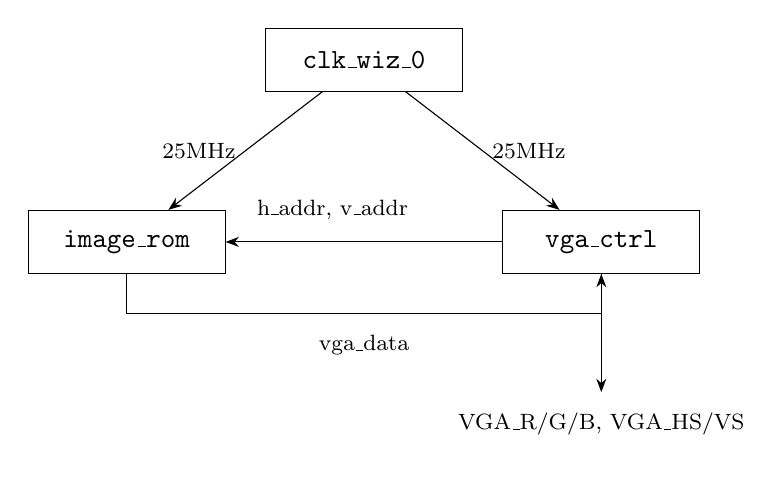
\begin{tikzpicture}[>=Stealth, node distance=1.8cm,
        every node/.style={draw, minimum width=2.5cm, minimum height=0.8cm}]
        \node (clk) {\texttt{clk\_wiz\_0}};
        \node[below right=1.5cm and 0.5cm of clk] (vga) {\texttt{vga\_ctrl}};
        \node[below left=1.5cm and 0.5cm of clk] (rom) {\texttt{image\_rom}};
        \node[below=1.5cm of vga, draw=none, minimum width=0pt, font=\footnotesize] (out) {VGA\_R/G/B, VGA\_HS/VS};
        \draw[->] (clk) -- node[right, draw=none, minimum width=0pt, font=\footnotesize] {25MHz} (vga);
        \draw[->] (clk) -- node[left, draw=none, minimum width=0pt, font=\footnotesize] {25MHz} (rom);
        \draw[->] (vga.west) -- +(-0.8,0) |- node[above, draw=none, minimum width=0pt, font=\footnotesize, near end] {h\_addr, v\_addr} (rom.east);
        \draw[->] (rom.south) -- +(0,-0.5) -| node[below, draw=none, minimum width=0pt, font=\footnotesize, near start] {vga\_data} (vga.south);
        \draw[->] (vga) -- (out);
    \end{tikzpicture}
    \caption{VGA 显示系统整体架构}
    \label{fig:top}
\end{figure}

板子上的 100MHz 时钟先经过 Clocking Wizard 分频到 25MHz
（VGA 标准要求的像素时钟），然后 VGA 控制器负责产生扫描坐标，
把坐标拼成地址去 ROM 里查像素数据，最后输出到 VGA 接口。

\subsection{VGA 时序控制}

\texttt{vga\_ctrl} 模块用 \texttt{x\_cnt} 和 \texttt{y\_cnt} 
两个 10 位计数器分别追踪当前的行位置和场位置。通过比较计数器值和各区间的边界，
就能得到 \texttt{hsync}、\texttt{vsync} 同步信号以及 \texttt{valid} 有效显示标志。
在有效区域内，模块会输出对应的行地址 \texttt{h\_addr} 和列地址 \texttt{v\_addr}，
在无效区域则输出全零。

当 \texttt{valid} 为高时，12 位的像素数据被拆成高 4 位、中 4 位、
低 4 位分别送到 \texttt{VGA\_R}、\texttt{VGA\_G}、\texttt{VGA\_B}；
无效区域则输出黑色（全零）。

\subsection{显存设计}

显存采用 Vivado 的 Block Memory Generator IP 核，配置为单口 ROM 模式，
数据宽度 12 位，深度 327\,680（即 $640 \times 512$）。
这里采用了讲义上的方法给每列分配了 512 行而不是 480 行，
这样可以直接把 \texttt{h\_addr} 的 10 位和 \texttt{v\_addr} 的低 9 位拼起来
得到 19 位地址，不用做额外的乘法或复杂的地址映射。

\subsection{时钟分频}

直接用代码实现时钟分频稳定性不足，这里使用 Clocking Wizard IP 核进行分频，
以下代码为生成 IP 核的 Tcl 脚本

\begin{lstlisting}
create_ip -name clk_wiz -vendor xilinx.com -library ip -version 6.0 -module_name clk_wiz_0 -dir $IP_DIR
set_property -dict [list \
    CONFIG.PRIM_IN_FREQ {100.000} \
    CONFIG.CLKOUT1_REQUESTED_OUT_FREQ {25.000} \
    CONFIG.USE_LOCKED {false} \
    CONFIG.USE_RESET {false} \
] [get_ips clk_wiz_0]
generate_target all [get_ips clk_wiz_0]
synth_ip [get_ips clk_wiz_0]
\end{lstlisting}

\subsection{自定义图片转换}

拓展要求是显示一张自己的图片。为此修改了提供的脚本 \texttt{coe\_generate.py}，
用 PIL 库读取图片，先 resize 到 640$\times$480，然后按列优先顺序遍历每个像素，
取 R、G、B 各通道的高 4 位拼成一个 12 位的十六进制值，写入 \texttt{.coe} 文件。
对于 480 到 511 行的 padding 区域，直接填零。

\section{实验总结与反思}

这次实验的主要工作量其实在于理解 VGA 时序和显存的地址映射关系。VGA 时序本身不复杂，
主要是参数较为复杂，我最开始没有看懂实验手册中的设计，弄混了很多次才最终完成。

看到自己的图片显示在屏幕上还是挺有成就感的。我原以为像 VGA 这种已经有点古老的技术，
可能显示效果不太好，没想到颜色和清晰度都还挺不错的。

\end{document}